\clearpage

\section{Codify ILP in MatLab}
\begin{tcolorbox}	
\begin{tabular}{p{2.75cm} p{0.2cm} p{10.5cm}} 	
\textbf{Student Name}  &:& Tiago Esteves        (November 28, 2017 - December 05, 2017)\\
\textbf{Goal}          &:& Help other to install lpsolve for using in MatLab.
\end{tabular}
\end{tcolorbox}
\vspace{17pt}

The first step to do as we can see in the image \ref{first_step} is to define the number of nodes in our network, create the matrices ODU for our traffic and then create a vector with the number of amplifiers in our network. In relation to the latter, the number of amplifiers is calculated through the distances between the nodes. These distances can be obtained through the matrix created initially but since it is a symmetric matrix we just need to use the upper matrix to create this vector.\\

\begin{figure}[h!]
\centering
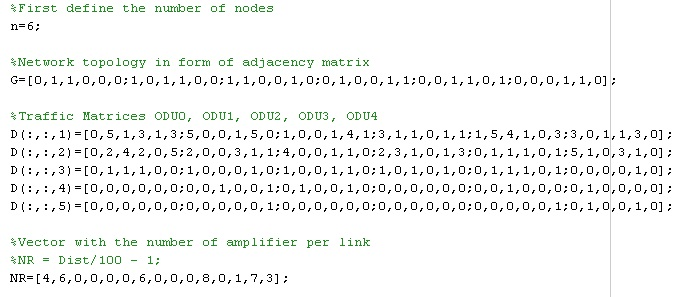
\includegraphics[width=\textwidth]{appendices/lpsolve/figures/first_step}
\caption{Number of nodes, matrices of ODU and number of amplifiers.}
\label{first_step}
\end{figure}

\vspace{13pt}
Following the code we can observe several cost variables with their respective values that will be necessary for the following calculations.\\
The next step can be observed in the image \ref{second_step}, where in this part we have to define the number of variables used in the constraints the total of these variables and also to create the ilp with these variables. As you can see in the image, each variable is calculated differently because each variable has a different value. Ilp is created using the 'make\_lp' function of mxlpsolve.\\
\newpage
\begin{figure}[h!]
\centering
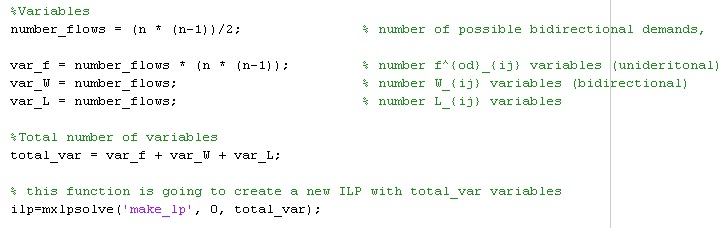
\includegraphics[width=\textwidth]{appendices/lpsolve/figures/second_step}
\caption{Number of variables, total number of variables and create ilp.}
\label{second_step}
\end{figure}

\vspace{13pt}
Through the image \ref{third_step} we can see how the objective function defined in section \ref{ILP_Opaque_Survivability} (Opaque without survivability) is encoded. The first thing to do for coding the objective function is to create a vector (f\_row) with the total number of variables, then for each position of a given variable we have to assign its corresponding value. This value is seen through the equation \ref{Capex}. Finally, using the 'set\_obj\_fn' function of mxlpsolve the objective function is defined.\\

\begin{figure}[h!]
\centering
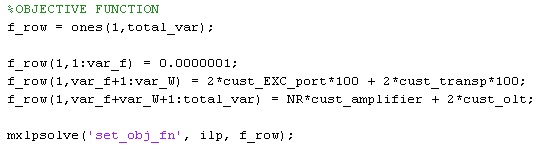
\includegraphics[width=\textwidth]{appendices/lpsolve/figures/third_step}
\caption{Objective function.}
\label{third_step}
\end{figure}

\vspace{13pt}
After defining the objective function we have to code all the necessary restrictions for the mode of transport in question. In the image \ref{four_step} we can see the first restriction referred to in section \ref{ILP_Opaque_Survivability}.
The use of the first two cycles 'for' is related to the fact that it has to be applied to all $o$ with $o$ being greater than $d$. The other two case 'for' refers to the fact that it is for all $i$ and for all $f$ where $i$ is equal to $o$, hence the use of an 'if' in between these two 'for'. Thus, it is only necessary to have an if loop for the case of $f$ to be different from $o$ because this $f$ is different from the origin. As this constraint refers to variable $f_{ij}^{od}$ f\_index is used where this variable is equal to the value calculated by the function index\_calculation2. Finally, the 'add constraint' function of mxlpsolve is used to add this constraint indicating that position (f\_row) must be equal (3) to 1.\\

\begin{figure}[h!]
\centering
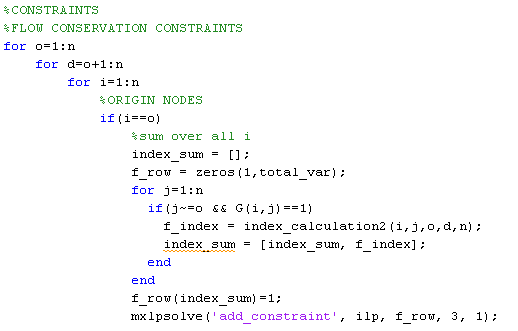
\includegraphics[width=\textwidth]{appendices/lpsolve/figures/four_step}
\caption{First constraint of this model.}
\label{four_step}
\end{figure}

\vspace{13pt}
After all the restrictions on the mode of transport in question have been codified, it is necessary to define the variables. As we can see in the image \ref{five_step} for the case of section \ref{ILP_Opaque_Survivability} (Opaque without survivability) the variables 'var\_f' and 'var\_L' are binary and the variable 'var\_w' is integer. Finally we use the 'write\_lp' function of mxlpsolve to write ilp to a file and the 'solve' function of mxlpsolve to solve this ilp.\\

\begin{figure}[h!]
\centering
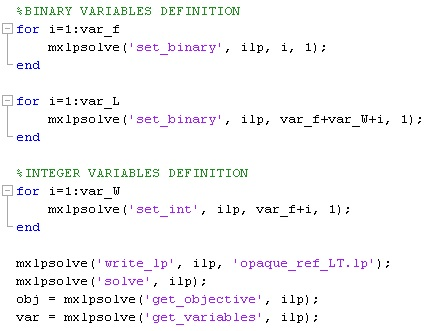
\includegraphics[width=\textwidth]{appendices/lpsolve/figures/five_step}
\caption{Definition of variables, write and solve the ilp.}
\label{five_step}
\end{figure}

Finally, only code is made to display the results in detail using 'fprintf' and creating variables to store the calculated values.\\

